%!TEX root = ../intro.tex
%******************************
%	 Other applications of scRNAseq
%*****************************

\section{General applications of scRNA-Seq in biology}

The following section outlines the applications of scRNA-Seq to a broad spectrum of biological systems. Whole transcriptomic read-outs of individual cells allowed the in-depth characterisation of embryonic development, haematopoiesis, immune responses, the detection of rare cell types and have led to new insights into disease progression including cancer development. 

\subsection{Atlas-type approaches}

Until recently, scRNA-Seq technologies generated transcriptomes of less than one thousand cells to study cell type heterogeneity, allele-specific expression or pseudo-temporal trajectories in cellular systems \citep{Kolodziejczyk2015review}. With the increased scalability of scRNA-Seq technologies, cellular composition of whole tissues and organisms can be assayed. The largest of these so called "expression atlases" to date is the 10X Genomics\textsuperscript{\textregistered}{} brain dataset comprising 1.3 million cells from embryonic mice. It was generated using 133 libraries sequenced on 11 Illumina HiSeq\textsuperscript{\textregistered}{} 4000 flowcells \citep{10XGenomics2017}. This experiment has been performed to exemplify the applicability of the commercial 10X Genomics platform to generate more than 10 billion transcriptomes of individual cells across the human body as envisioned by the Human Cell Atlas Consortium \citep{Regev2017}.\\

So far, transcriptional atlases that comprise thousands of cells include the mouse cell atlas, a thymus organogenesis atlas, an ageing lung atlas and the full characterisation of cell types in \textit{C. elegans}. For example, Microwell-Seq was developed to capture more than 400,000 cells covering all mouse organs. This analysis reveals rare cell types such as 2-cell-stage like mESCs and allows the construction of a cross-tissue correlation network \cite{Han2018}. Similarly, the \emph{Tabula Muris} aimed at detecting all major cell type across 20 organs of the mouse. Here, the Tabula Muris Consortium used droplet-based 3'-end scRNA-Seq and FACS-based full length transcript analysis to generate (i) a broad atlas and (ii) an in-depth characterisation of each tissue \citep{Quake2018}. Cao \emph{et al.}, 2017 generated more than 40,000 cells from the L2 stage \emph{C. elegans} using sci-RNA-Seq and identified nineteen distinct cell types and seven mixed cell types. Furthermore, this atlas allows the dissection of neuronal cell types that split across seven clusters \citep{Cao2017}. To study thymus development, Kernfeld \emph{et al.}, 2018 generated around 25,000 transcriptomes of individual cells from the embryonic thymus at E12.5, E13.5, E14.5, E15.5, E16.5, E17.5, E18.5, and P0. This experimental set-up resolves the temporal development of immune cell types such as T cells, myeolid cells, natural killer cells, innate lymphoid cells, and $\gamma{}\delta{}$ T cells as well as thymic epithelial cells \citep{Kernfeld2018}. Finally, to study the effect of ageing on a whole tissue, Angelidis \emph{et al.}, 2018 isolated 14,000 cells from lungs of young and old animals and found (i) an increase in transcriptional noise during ageing and (ii) altered transcriptional profiles of alveolar macrophages and type 2 pneumocytes \citep{Angelidis2018}.\\

The following paragraphs summarise scRNA-Seq applications that are aimed at more targeted analysis of regulatory processes.

\subsection{Developmental biology}

Over the last few years, the development of new scRNA-Seq technologies and algorithms to perform data analysis uncovered driving factors in development and cell fate decisions \citep{Griffiths2018}. An early study of mouse embryonic development identified that transcriptional differences between the two cells in the 2-cell stage embryo increase from the zygote to late 2-cell stage embryos. This is caused by an initial partitioning "error" where transcripts are unevenly distributed between the daughter cells. Later on, these differences are strengthened by the onset of transcription coupled to transcriptional noise \citep{Piras2014, Shi2015a}. A reproducible distribution of transcripts in the first cell division was also detected by Biase \emph{et al.}, 2014 \cite{Biase2014}. These biases between cells at the 2-cell stage propagate to form transcription biases at the 4-cell pushing cells towards forming the pluripotent inner cell mass or the extra-embryonic trophoectoderm \citep{Goolam2016, Shi2015a}. To obtain a more complete view on gastrulation in the mouse, Scialdone \emph{et al.} captured cells from the epiblast at E6.5 and mesodermal cells at E7.0, E7.5 and E7.75. The authors also sampled cells from \emph{Tal1} knock-out animals and showed that this transcription factor is a key regulator for blood develeopment \citep{Scialdone2016}. \\

This year, large-scale scRNA-Seq studies profiled organogenesis in the mouse and zebrafish. Ibarra-Soria \emph{et al.}, 2018 sampled more than 20,000 cells from E8.25 embryos following gastrulation and identified 20 major cell types including different mesoderm lineages, neural progenitor cells, blood, gut and extra-embryonic cells. They further used this data to dissect gut formation and to find oscillating expression patterns during somitogenesis \citep{Ibarra-Soria2018}. Similarly, inDrop and Drop-Seq approaches were used to generate $\sim$7000 cells from \gls{Dmelanogaster} embryos at the onset of gastrulation \citep{Karaiskos2017} or to generate more than 90,000 cells from the zebrafish embryo during the first day of development \citep{Wagner2018}.\\

In the last two years, experimental procedures were developed to track cells across multiple divisions termed "lineages". For this, the genome editing tool: \gls{CRISPR}/\gls{Cas9} \citep{Jinek2012}, was used to introduce so called "scars" at specific DNA sequences. In bacteria, the CRISPR/Cas system is used to degrade invasive DNA which involves a CRISPR RNA that recognises the invading DNA and a Cas protein for degradation. For genome editing purposes, the \gls{CRISPR}/\gls{Cas9} uses \glspl{sgRNA} to specific genomic sites and induces \gls{DSB}. Upon repair, insertions or deletion mutations are introduced that render a specific gene non-functional \citep{Zhang2014c}. The first approach to use the 	\gls{CRISPR}/\gls{Cas9} for scarring: \gls{GESTALT}, inserted an array of 10 \gls{CRISPR}/\gls{Cas9} with variable specificity into the genome of individual cells. Upon the expression of the Cas9 protein and the \gls{sgRNA}, random scars are introduced into the genomic array. After days of growth, genomic DNA was harvested and the array was sequenced to construct the relationship between individual cells \textbf{(Fig.~\ref{fig0:CRISPR})} \citep{McKenna2016}. This technology has been extended as a scRNA-Seq approach to capture the RNA together with the expressed \gls{CRISPR}/\gls{Cas9} array that allows cell type assessment alongside lineage detection. This approach also includes a heat shock inducible system to start the scarring at later stages of development \citep{Raj2018}. Similar approaches used multiplexed smFISH read-outs to infer lineage relationship between individual cells \citep{Frieda2017} or tranposase-based insertion of a random 20mer sequence into the genome \citep{Wagner2018}.\\

One current challenge, especially in the field of developmental biology, is to obtain spatially-resolved whole-transcriptome read-outs of individual cells. The imaging technologies introduced above, MERFISH and SeqFISH, are capable of capturing single RNA molecules of thousands of genes across thousands of cells. Early approaches in the field of spatial transcriptomics employed spatial gene expression atlases to map isolated single cells back into the tissue of origin \citep{Achim2015, Satija2015a}. A similar approach has recently been used to spatially locate cells isolated form the \gls{Dmelanogaster} embryo \citep{Karaiskos2017}. Moreover, Tomo-Seq was developed to sequence RNA extracted from slices of the zebrafish embryos. RNA was extracted from each slice into a tube and barcoded prior to sequencing. Matched histology and mathematical modelling was used to reconstruct the spatial expression patterns across the embryo \citep{Junker2014a}.

\begin{figure}[!h]
\centering
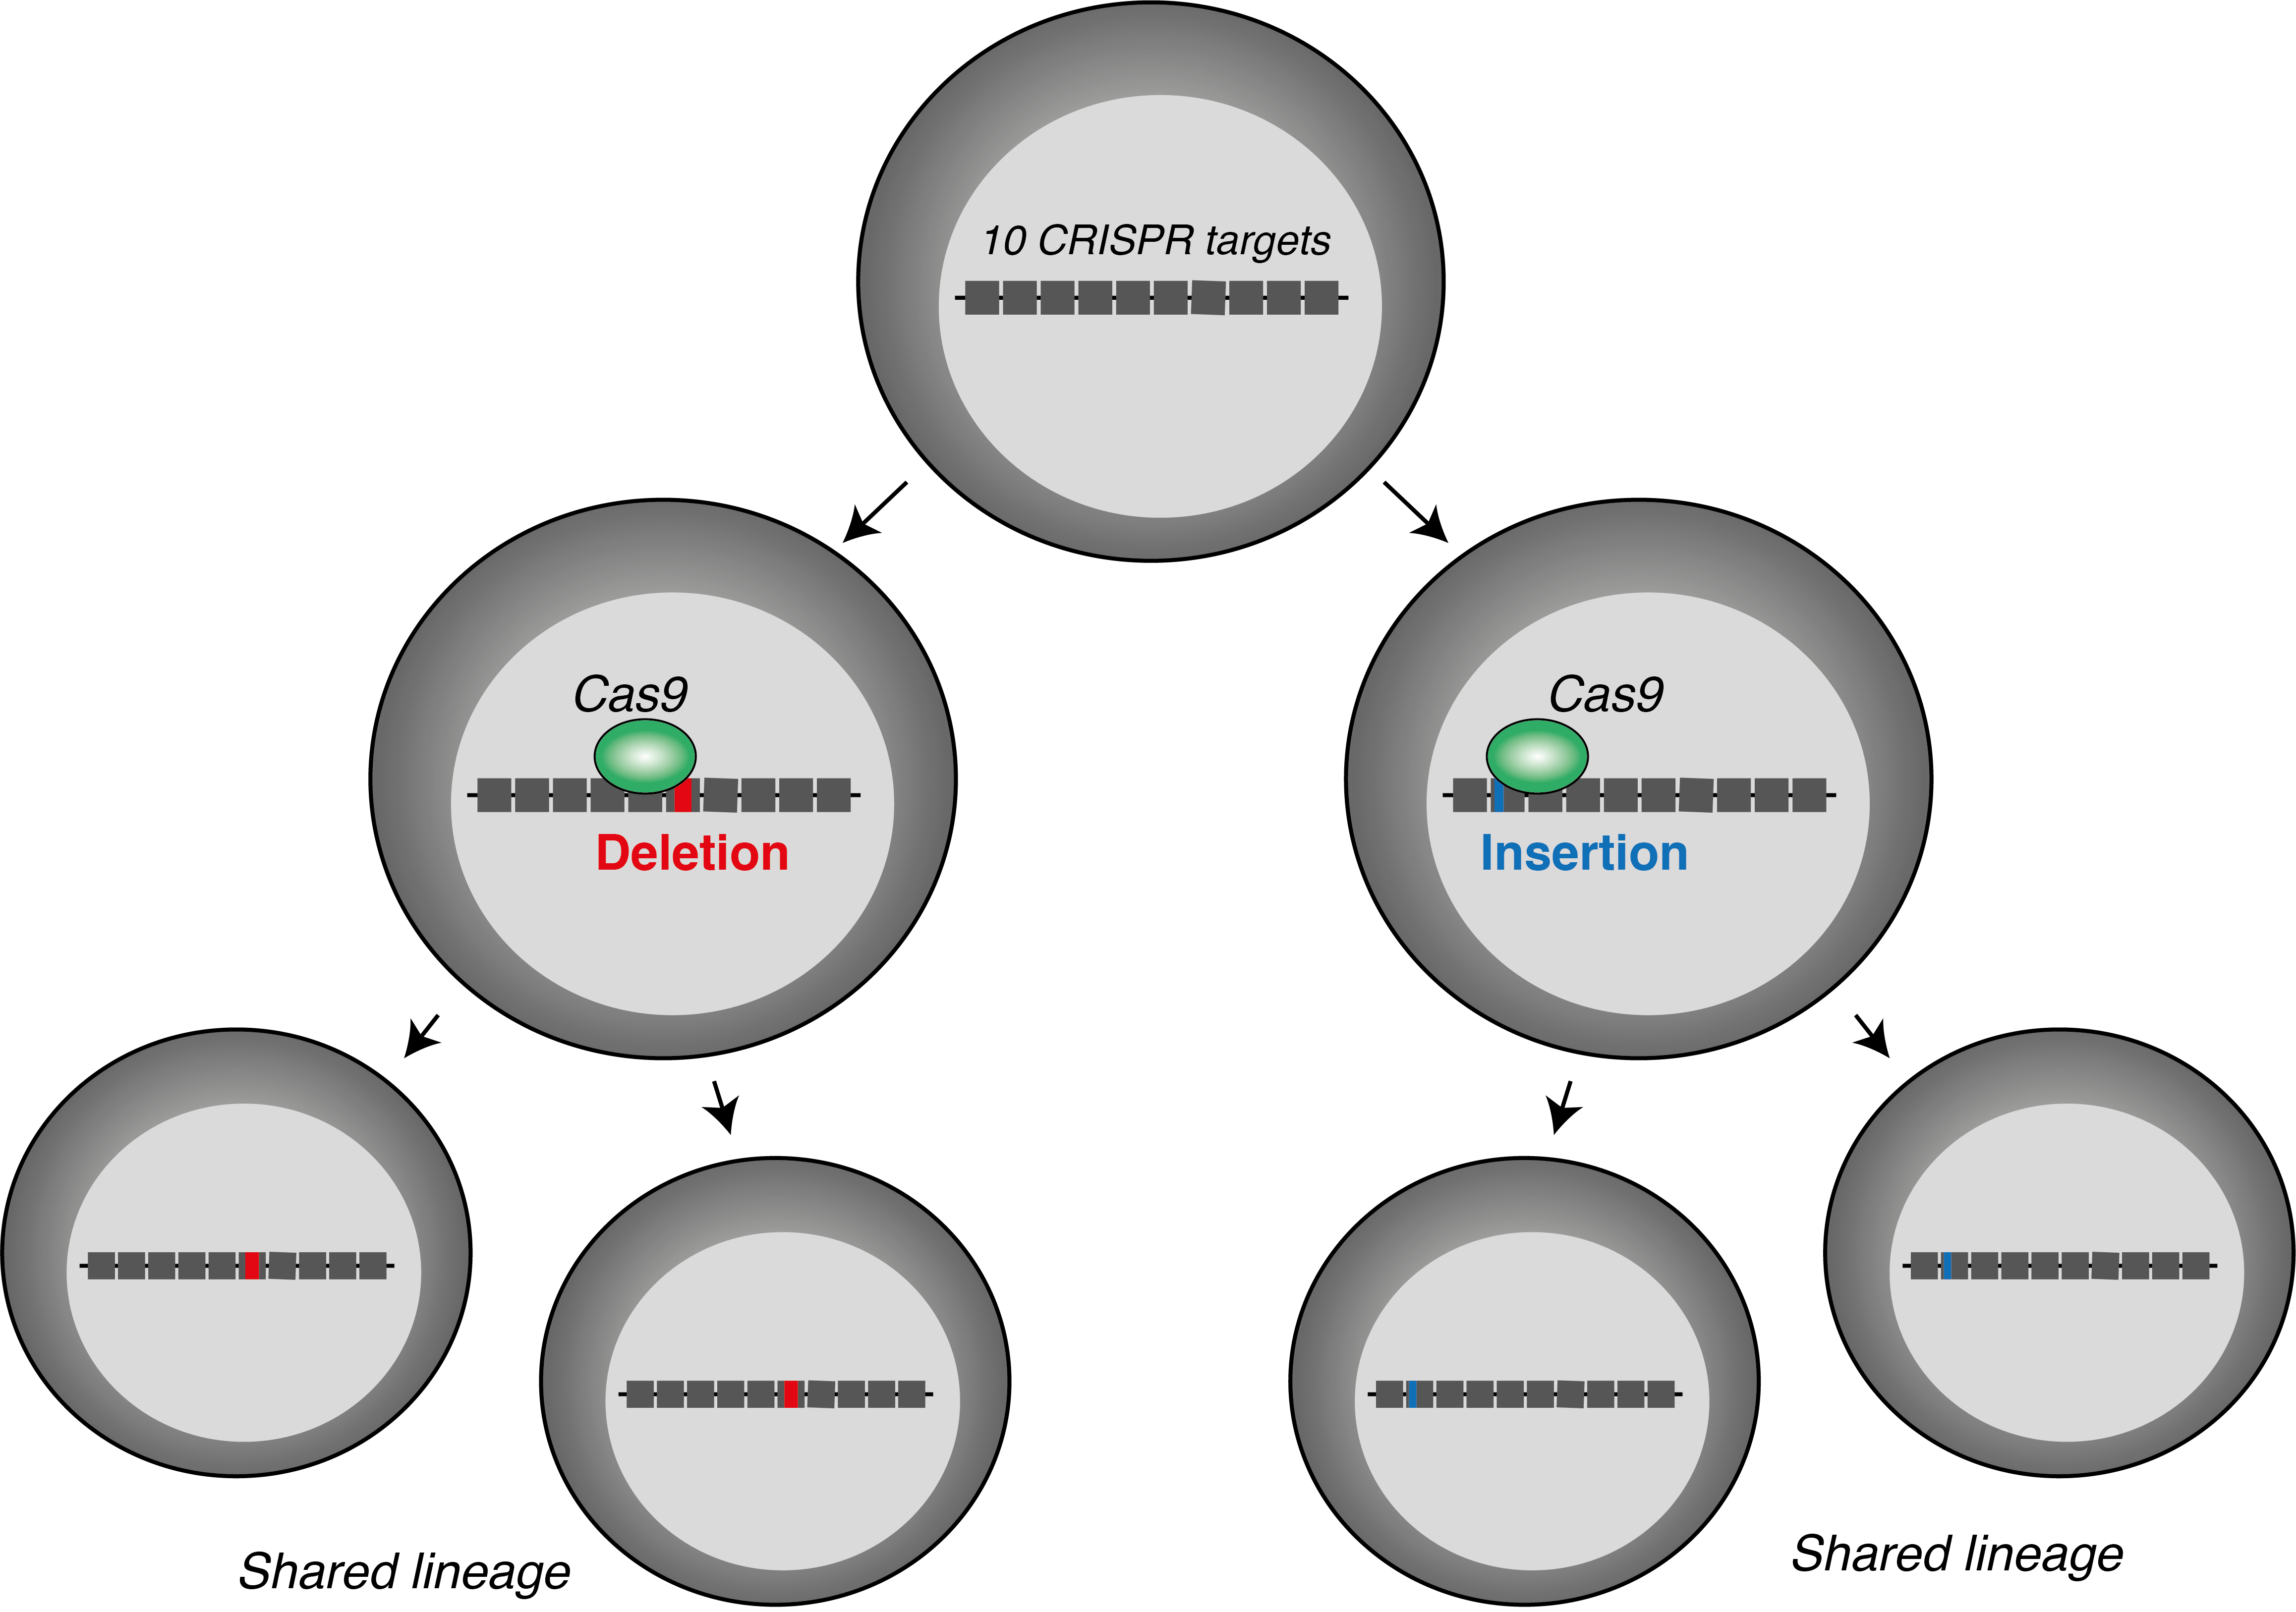
\includegraphics[width=\textwidth]{Fig_17.png}
\caption[CRISPR/Cas9-scarring for lineage tracing]{\textbf{CRISPR scarring for lineage tracing.}\\
A cassette of 10 CRISPR targets is inserted into the genome. Upon Cas9 expression, random insertions and deletions are added to these cassettes. Single-cell DNA or RNA sequencing allows detecting the scars and therefore cell lineage reconstruction.}
\label{fig0:CRISPR}
\end{figure}

\subsection{Cell type evolution} 

Evolutionary biology is a research field that less frequently uses scRNA-Seq approaches to understand the evolutionary origin of cell types. To do this, cell compositions of non-model organisms such as \gls{Pdumerilii} (annelid), \gls{Nvectensis} (cniderian), \gls{Aqueenslandica} (sponge), \gls{Mleidyi} (ctenophore) and \gls{Tadhaerens} (placozoan) are compared. All of these organisms (except annelids) are non-bilaterians and therefore evolutionary older than mouse and humans. As an example and part of an early project, we used the developing larva of \textit{P. dumerilii} to study diversification of cell types in early bilaterian evolution. We detected cells from the apical neuroectoderm, the midgut, striated musculatrue, ciliated cells and non-apical blastopore cells. By assessing the transcriptional distance between these cell types, we formulated a hypothesis of related cell type families that originate from an ancesteral cell type and are conserved during evolution \citep{Achim2018}.  \\

Seb\'e{}-Pedr\'o{}s \emph{et al.}, 2018 generated a single-cell expression atlas of adult and larval \textit{N. vectensis} using MARS-Seq. This dataset allowed the dissection of neuronal diversification and transcription factor regulatory programmes in this early sister group of bilaterians \citep{Sebe-Pedros2018}. The authors furthermore generated similar atlases of \textit{A. queenslandica}, \textit{M. leidyi} and \textit{T. adhaerens} and performed cross-species gene module analysis after cell type identification. Co-regulation of cell type-specific gene modules strongly diverged between the species except for a few house keeping modules. Moreover, regulatory TF modules appear to be cell type and species-specific \citep{Sebe-Pedros2018a}. These studies highlight scRNA-Seq as a powerful tool to study inter-species relationships of cell types in non-model organisms. 

\subsection{Immunology}

The immune system has been extensively studied using scRNA-Seq to detect activation responses and to dissect the transcriptional heterogenity among immune cells \citep{Proserpio2015, Satija2014}. White blood cells are broadly grouped into cells of the innate and adaptive immune system. Innate immune cells (\gls{DC}, mast cells, macrophages, basophils, neutrophils, \gls{NK} cells, eosinophils) are fast responders that represent the first line of defence upon infection. The adaptive immune system (B cells, CD4\plus{} and CD8\plus{} T cells) responds more slowly but installs an antigenic specificity and immune memory after infection. \gls{NK} T cells and \textgamma{}\textdelta{} T cells are cytotoxic lymphocytes that show both innate and adaptive characteristics \textbf{(Fig.~\ref{fig0:immune_system})} \citep{Dranoff2004}. 

\begin{figure}[!h]
\centering
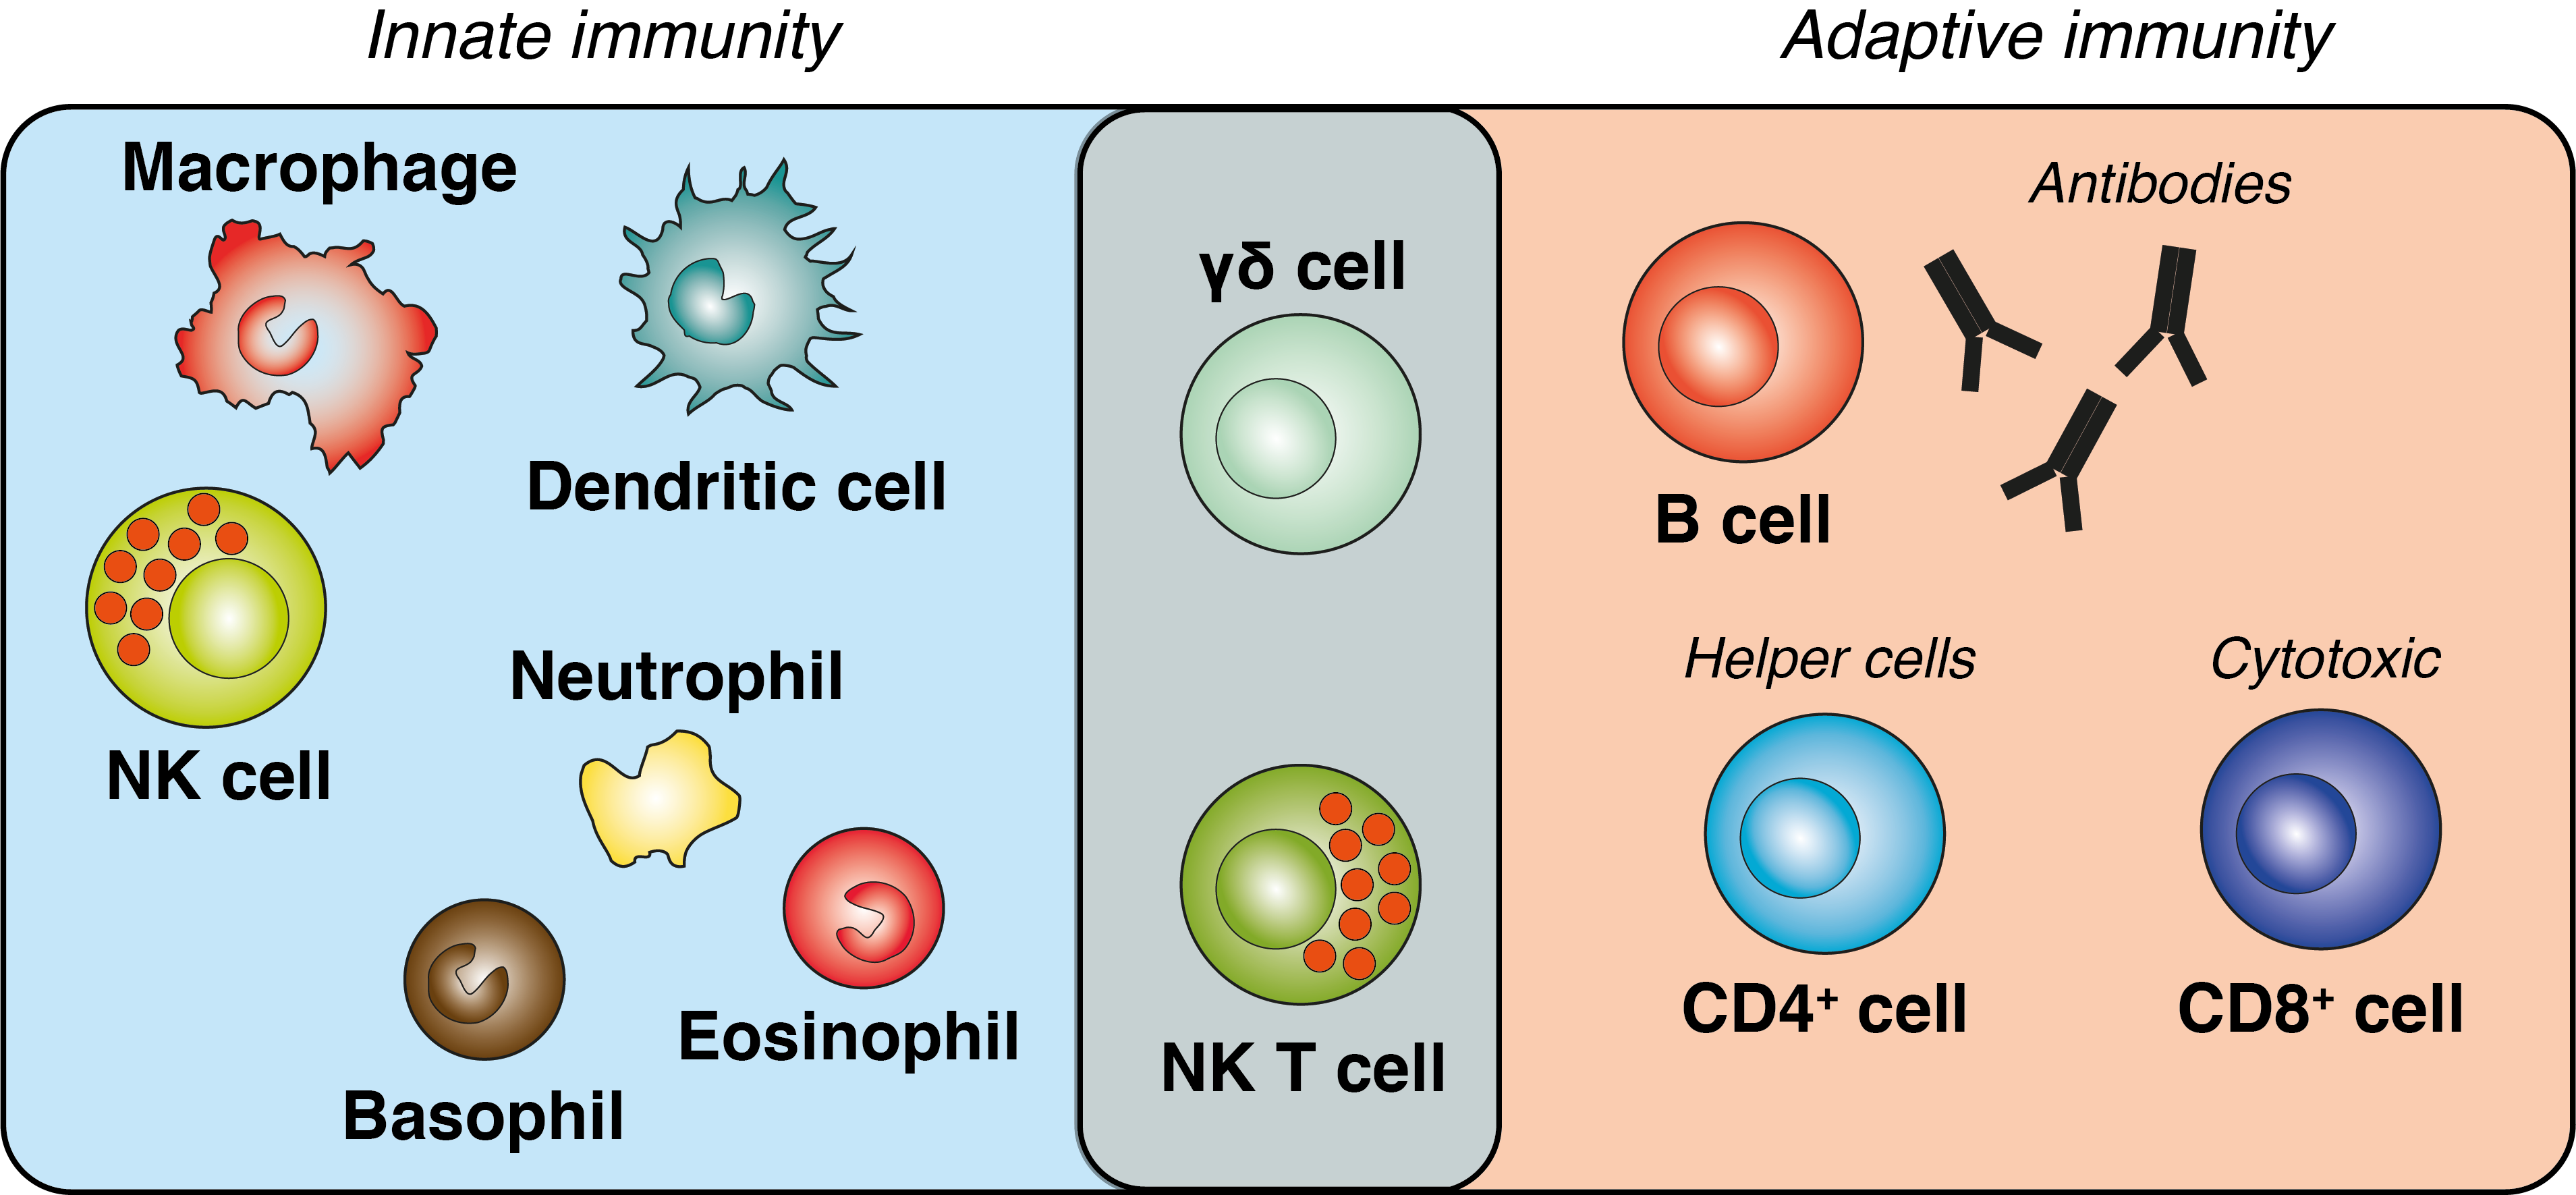
\includegraphics[width=\textwidth]{Fig_18.png}
\caption[Cell types of the adaptive and innate immune system]{\textbf{Cell types of the adaptive and innate immune system.}}
\label{fig0:immune_system}
\end{figure}

An unbiased approach analysed $\sim$65,000 human \glspl{PBMC} and identified the major innate and adaptive immune cell types. The authors further used droplet-based scRNA-Seq to study bone marrow mononuclear cells after haematopoietic stem cell transplant in an \gls{AML} patient. The technology allowed the distinction between host and donor cells and the detection of residual AML cells in the host \citep{Zheng2017}. \\

More targeted approaches focused on either cells of the innate or adaptive immune system.

\subsubsection{scRNA-Seq to study innate immunity}

Villani \emph{et al.}, 2017 used plate-based scRNA-Seq to dissect the \gls{DC} and monocyte compartment of human \glspl{PBMC}. In general, DCs can be subdivided into CD11C\plus{} conventional DCs (CD141\plus{} and CD1C\plus{}) that activate CD4\plus{} and CD8\plus{} and interferon producing, plasmacytoid DCs. Monocytes were classically subdivided into CD14\plus{} and CD16\plus{} cells. After analysing more than 2,400 DCs and monocytes, the authors expanded DCs to consist of 6 groups and detected conventional DC progenitor cells. Furthermore, they detected two new groups of uncharacterised monocytes \citep{Villani2017}. Shalek \emph{et al.}, 2014 used the Fluidigm C1 system to generate transcriptomes of more than 1700 primary mouse bone marrow derived DCs to study their activation response during \gls{LPS} stimulation. Within one hour of activation, early responding cells up-regulate \gls{Ifn}\textbeta{} and support the activation of surrounding cells via paracrine signalling. By isolating activated cells in individual chambers, the authors showed a decrease in the total number of activated cells after 4h stimulation with LPS. Furthermore, activated cells need autocrine stimulation to fully activate and Ifn\textbeta{} secretion during the first hour of activation is the crucial trigger for homogeneous DC activation \citep{Shalek2014}. Bj\"o{}rklund \emph{et al.}, 2016 performed targeted scRNA-Seq of Lin\textsuperscript{-}CD127\plus{} \glspl{ILC} and NK cells from tonsil tissue of adult humans using the SmartSeq2 protocol. They firstly identified the three major lineages of ILCs (ILC1, ILC2 and ILC3) and further assessed heterogeneity within the ILC3 population. Dissecting this rare cell type allows a deeper understanding of immune regulation in humans \citep{Bjorklund2016}. 

\subsubsection{scRNA-Seq to study adaptive immunity}

The majority of scRNA-Seq studies focused on dissecting heterogeneity in the CD4\plus{} or CD8\plus{} T cell compartment to understand adaptive immunity. For example, Proserpio \emph{et al.}, 2016 studied CD4\plus{} Th2 cell differentiation after \textit{Nippostrongylus brasiliensis} infection. 5 days after infection, three major cell states can be detected: (i) activated cells, (ii) proliferating cells and (iii) Th2 cytokine expressing cells. Furthermore, more differentiated, cytokine-producing cells show higher proliferation which was validated by an \emph{in vivo} model of Th1 differentiation upon malaria infection \citep{Proserpio2016}. A follow-up study characterised the time course of malaria infection by sampling labelled CD4\plus{} T cells 2, 3, 4 and 7 days after infection. Gaussian process modelling of expression changes over the differentiation time course revealed a bifurcation between the Th1 and \gls{Tfh} cell lineage. Identifying such branching dynamics during cell differentiation allows the characterisation of decision-making molecules and underlying regulatory mechanisms \citep{Lonnberg2017}. \\

Prior to differentiation and to trigger activation responses, the \gls{TCR} on T cells recognises peptides bound to \gls{MHCI} molecules on an antigen-presenting cell (e.g.~DC). Upon peptide recognition and co-activator stimulation, cytoskeletal rearrangements, metabolic changes and transcription-factor activity lead to the proliferation and effector differentiation of T cells \citep{Richard2018}. Richard \emph{et al.}, 2018 studied the effects of reduced TCR-peptide affinity and discovered that CD8\plus{} cells show heterogeneous response patterns to stimulation with low-affinity peptides. Nevertheless, once activated, CD8\plus{} T cells reach similar activation stages compared to cells activated with high-affinity peptides \citep{Richard2018}. Similar to the differentiation time course experiments using CD4\plus{} T cells, Kakaradov \emph{et al.}, 2017 tracked expression changes over the differentiation course of CD8\plus{} T cells after lymphocytic choriomeningitis virus infection. The authors detected strong divergence during the first division of CD8\plus{} T cells after infection which is strengthened by epigenetic silencing of genes associated to memory formation \citep{Kakaradov2017}.\\

The development of scRNA-Seq technologies has also driven the expansion of tools to analyse single-cell transcriptome data. Key algorithms for T cell and B cell analysis include the reconstruction of the TCR and \gls{BCR}. Constructing the TCR of individual cells allows the identification of clonal expansion of CD4\plus{} T cells upon \textit{Salmonella} infection \citep{Stubbington2016}. Similarly, the BCR can be reconstructed to detect clonal heterogeneity in B cell populations \citep{Canzar2017, Wu2018}

\subsection{Tissue function and disease}

One example for scRNA-Seq applications to study tissue functions is the work by Sten Linnarsson's lab that aims at dissecting the complexity of the mammalian brain. In an early study, Zeisel \emph{et al.}, 2015 sequenced $\sim$ 3000 cells from the mouse somatosensory cortex and hippocampal \gls{CA}1 region and identified a variety of interneurons, S1 pyramidal neurons, CA1 pyramidal neurons, mural cells, endothelial cells, microglia cells, ependymal cells, astrocytes and oligodendrocytes \citep{Zeisel2015}. More recently, H\"a{}ring \emph{et al.}, 2018 studied sensory neurons in the dorsal horn of mice and detected multiple sub-groups of \gls{GABA}ergic and glutamatergic neurons \citep{Haring2018}. A large-scale study of more than 500,000 cells of the mouse nervous system generated an atlas comprising all major neuronal and non-neuronal cell types. For this, cells from anatomical units of the brain as well as cells from the spinal cord, dorsal root ganglia, sympathetic ganglion and the enteric nervous system were sampled \citep{Zeisel2018}. On a smaller scale, Davie \emph{et al.}, 2018 generated an atlas of 57,000 cells from the \gls{Dmelanogaster} brain from young and old animals \cite{Davie2018}.\\

Bach \emph{et al.}, 2017 used droplet-based scRNA-Seq to dissect the development of the adult mammary gland. By sampling cells from the mammary gland at different time points (8 weeks virgin, 14.5 days gestation, 6 days lactation and 11 days post involution), the authors were able to reconstruct differentiation processes including the development of hormone-sensing and secretory cells \citep{Bach2017}. To study the spatial expression pattern of the liver, Halpern \emph{et al.}, 2017 mapped scRNA-Seq profiles onto 9 layers around the central vein. This approach allows the detection of novel gene expression patterns that correlated with the distance of the cell layer to the central vein \citep{Halpern2017}. Young \emph{et al.}, 2018 generated 70,000 single-cell transcriptomes from human renal tumours as well as healthy foetal, pediatric, and adult kidneys. With this data, the authors linked childhood Wilms tumour to abnormal foetal cells and identified precursor cells for adult tumours \citep{Young2018}. \\

Extending this, scRNA-Seq was used to study malignant tumours where full characterisation is hindered by complex cellular heterogeneity. Early work by Patel \emph{et al.}, 2014 identified strong heterogeneity within glioblastomas of five patients related to oncogenic signalling, proliferation, immune response, and hypoxia. Furthermore, within each tumour, cells are classified as different glioblastoma sub-types which potentially complicates treatment strategies \citep{Patel2014}. More recently, scRNA-Seq has been performed to dissect the multicellular ecosystems of metastatic melanoma \citep{Tirosh2016} and head and neck cancer \citep{Puram2017}. In both studies, malignant cells clustered patient-dependently and non-malignant cells clustered based on their cell type. These studies highlight the extreme transcriptional heterogeneity within and between tumours which complicates standard therapies. \\

